\documentclass[../practica.root.tex]{subfiles}

\begin{document}

\section{Unidad 3}

\begin{enumerate}
  \item Usted realiza un trabajo de medio tiempo, y un supervisor le pide traer del almacén una varilla cilíndrica de acero de \SI{85,8}{\cm} de longitud y \SI{2,85}{\cm} de diámetro. ¿Necesita usted un carrito? (Para contestar, calcule el peso de la varilla)

        Dato: $\delta_{Acero}= \SI{7,80e3}{\kilogram\per\meter\cubed}$

        \[V=\pi\cdot r^2\cdot h\]
        \[V=\pi\cdot(\SI{1,43}{\cm})^2\cdot\SI{85,8}{\cm}\]
        \[V=\pi\cdot(\SI{0,0143}{\meter})^2\cdot\SI{0,858}{\meter}\]
        \[V=\SI{5,51e-4}{\meter\cubed}\]
        \[\delta=\frac{M}{V}\]
        \[M=\delta V\]
        \[M=\SI{7,80e3}{\kilogram\per\meter\cubed}\cdot\SI{5,51e-4}{\meter\cubed}\]
        \[M=\SI{4,30}{\kilogram}\]
        \[P=Mg\]
        \[P=\SI{4,30}{\kilogram}\cdot\SI{9,80}{\meter\per\second\squared}\]
        \[P=\boxed{\SI{42,1}{\newton}}\]

  \item Una esfera uniforme de plomo y una de aluminio tienen la misma masa. ¿Cuál es la relación entre los radios de la esfera de aluminio y el de la esfera de plomo?

        Datos: $\delta_{Al}=\SI{2,70e3}{\kilogram\per\meter\cubed}$; $\delta_{Pb}=\SI{11,3e3}{\kilogram\per\meter\cubed}$

        \[M_{Al}=M_{Pb}=\SI{1000}{\kilogram}\]

        \begin{multicols}{2}
          \[\delta_{Al}=\frac{M_{Al}}{V_{Al}}\]
          \[\SI{2,70e3}{\kilogram\per\meter\cubed}=\frac{\SI{1000}{\kilogram}}{V_{Al}}\]
          \[V_{Al}=\frac{\SI{1000}{\kilogram}}{\SI{2,70e3}{\kilogram\per\meter\cubed}}\]
          \[V_{Al}=\SI{0,370}{\meter\cubed}\]
          \[V_{Al}=\frac{4}{3}\pi r_{Al}\]
          \[\SI{0,370}{\meter\cubed}=\frac{4}{3}\pi (r_{Al})^3\]
          \[\SI{0,0883}{\meter\cubed}=(r_{Al})^3\]
          \[\sqrt[3]{\SI{0,0883}{\meter\cubed}}=r_{Al}\]
          \[\SI{0,445}{\meter}=r_{Al}\]

          \[\delta_{Pb}=\frac{M_{Pb}}{V_{Pb}}\]
          \[\SI{11,3e3}{\kilogram\per\meter\cubed}=\frac{\SI{1000}{\kilogram}}{V_{Pb}}\]
          \[V_{Pb}=\frac{\SI{1000}{\kilogram}}{\SI{11,3e3}{\kilogram\per\meter\cubed}}\]
          \[V_{Pb}=\SI{0,0885}{\meter\cubed}\]
          \[V_{Pb}=\frac{4}{3}\pi r_{Pb}\]
          \[\SI{0,0885}{\meter\cubed}=\frac{4}{3}\pi (r_{Pb})^3\]
          \[\SI{0,0211}{\meter\cubed}=(r_{Pb})^3\]
          \[\sqrt[3]{\SI{0,0211}{\meter\cubed}}=r_{Pb}\]
          \[\SI{0,276}{\meter}=r_{Pb}\]
        \end{multicols}

        \[\frac{r_{Al}}{r_{Pb}}=\frac{\SI{0,445}{\meter}}{\SI{0,276}{\meter}}=\boxed{\num{1,61}}\]

  \item Un disco cilíndrico de madera que pesa \SI{45,0}{\newton} y tiene un diámetro de \SI{30,0}{\centi\meter} flota sobre un cilíndro de aceite cuya densidad es de \SI{0,850}{\gram\per\centi\meter\cubed} como muestra la figura. El cilíndro de aceite mide \SI{75,0}{\centi\meter} de alto y tiene un diámetro igual al cilíndro de madera.

        \begin{center}
          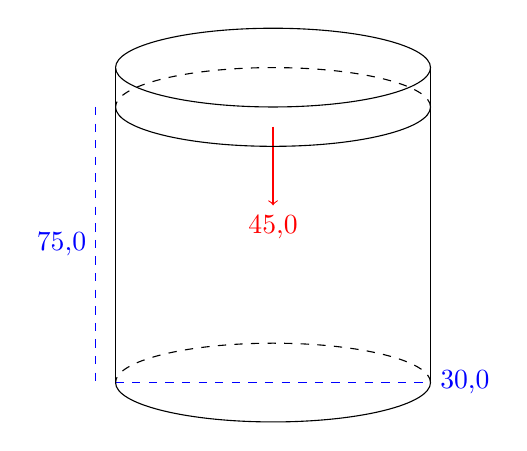
\begin{tikzpicture}
            \draw[dashed, blue] (-2,-4) -- ++(4,0) node[anchor=west]{\SI{30,0}{\centi\meter}};
            \draw[dashed, blue] (-2.25,-.5) -- ++(0,-3.5) node[pos=.5,anchor=east]{\SI{75,0}{\centi\meter}};
            \draw[red,->] (0,-.75) -- ++(0,-1) node[anchor=north]{\SI{45,0}{\newton}};
            \draw (0,0) circle [x radius=2, y radius=.5];
            \draw (-2,-.5) arc (180:360:2 and .5);
            \draw[dashed] (2,-.5) arc (0:180:2 and .5);
            \draw (-2,0) -- ++(0,-4);
            \draw (2,0) -- ++(0,-4);
            \draw (-2,-4) arc (180:360:2 and .5);
            \draw[dashed] (2,-4) arc (0:180:2 and .5);
          \end{tikzpicture}
        \end{center}

        \begin{enumerate}
          \item Calcule la presión manométrica en la parte superior de la columna de aceite.

                \[F_i=P_iA\]
                \[\SI{45,0}{\newton}=P_i\cdot\pi\cdot(\SI{0,150}{\meter})^2\]
                \[P_i=\frac{\SI{45,0}{\newton}}{\pi\cdot(\SI{0,150}{\meter})^2}\]
                \[P_i=\boxed{\SI{637}{\pascal}}\]

          \item Ahora suponga que alguin coloca un peso de \SI{83,0}{\newton} en la parte superior del disco de madera, pero el aceite no se escurre alrededor del borde de la madera.

                \begin{enumerate}
                  \item ¿Cuál es el cambio de presión en la base del aceite?

                        \[F_f=P_fA\]
                        \[\SI{45,0}{\newton}+\SI{83,0}{\newton}=P_f\cdot\pi\cdot(\SI{0,150}{\meter})^2\]
                        \[P_f=\frac{\SI{45,0}{\newton}+\SI{83,0}{\newton}}{\pi\cdot(\SI{0,150}{\meter})^2}\]
                        \[P_f=\SI{1,81e3}{\pascal}\]

                        \[\Delta P=P_f-P_i\]
                        \[\Delta P=\SI{1,81e3}{\pascal}-\SI{637}{\pascal}\]
                        \[\Delta P=\boxed{\SI{1,17e3}{\pascal}}\]

                  \item ¿Cuál es el cambio de presión a la mitad de la columna de aceite?

                        \[\SI{0,850}{\gram\per\centi\meter\cubed}\cdot\frac{\SI{1}{\kilogram}}{\SI{1000}{\gram}}\cdot\frac{(\SI{100}{\meter})^3}{\SI{1}{\cm\cubed}}=\SI{850}{\kilogram\per\meter\cubed}\]

                        \[\Delta P=P_f-P_i+\delta gh\]
                        \[\Delta P=\SI{1,81e3}{\pascal}-\SI{637}{\pascal}+\SI{850}{\kilogram\per\meter\cubed}\cdot\SI{9,80}{\meter\per\second\squared}\cdot\SI{0,375}{\meter}\]
                        \[\Delta P=\boxed{\SI{4,30e3}{\pascal}}\]
                \end{enumerate}
        \end{enumerate}

  \item Un cortocircuito deja sin electricidad a un submarino que está a \SI{30,0}{\meter} por debajo de la superficie del mar. Para escapar, la tripulación debe empujar hacia fuera una escotilla ubicada en el fondo, la cual tiene un área de \SI{0,750}{\meter\squared} y pesa \SI{300}{\newton}. Si la presión interior es de \SI{1,00}{atm}, ¿qué fuerza hacia abajo se debe hacer sobre la escotilla para abrirla?

        Dato: $\delta_{agua}=\SI{1,03e3}{\kilogram\per\meter\cubed}$

        \begin{center}
          \begin{tikzpicture}
            \draw[cyan,snake it] (-4,3) -- ++(7.5,0);
            \draw (-2.5,-1) rectangle(2.5, 1);
            \draw[red] (0,0) node{\SI{1,00}{atm}};
            \draw (-1,-1) ++(0,.25) -- ++(0,-.5);
            \draw (1,-1) ++(0,.25) -- ++(0,-.5);
            \draw[blue] (0,-1) node[anchor=south]{\SI{0,750}{\meter\squared}};
            \draw[dashed,blue,->] (-3,3) -- (-3,-1) node[pos=.5,anchor=east]{\SI{30,0}{\meter}};
            \draw[red,->] (0, -1) -- ++(0,-1) node[anchor=north]{\SI{300}{\newton}};
          \end{tikzpicture}
        \end{center}

        \[\SI{1,00}{atm}=\SI{1,01e5}{\pascal}\]

        \[\Delta P=\delta gh\]
        \[\Delta P=\SI{1,03e3}{\kilogram\per\meter\cubed}\cdot\SI{9,80}{\meter\per\second\squared}\cdot\SI{30,0}{\meter}\]
        \[\Delta P=\SI{3,03e5}{\pascal}\]

        \[F=PA\]
        \[F=\SI{3,03e5}{\pascal}\cdot\SI{0,750}{\meter\squared}\]
        \[F=\boxed{\SI{2,27e5}{\newton}}\]

        \newpage

  \item Un tubo en forma de U abierto por ambos extremos contiene un poco de mercurio. Se vierte un poco de agua en el brazo izquierdo del tubo hasta que la altura de la columna de agua es \SI{15,0}{\cm} como muestra la figura.

        Datos: $\delta_{Hg}=\SI{13,6e3}{\kilogram\per\meter\cubed}$; $\delta_{h2o}=\SI{1,00e3}{\kilogram\per\meter\cubed}$

        \begin{center}
          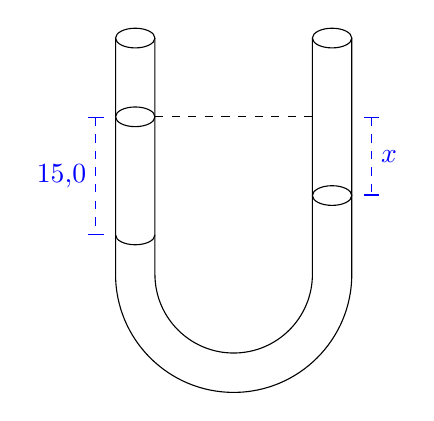
\begin{tikzpicture}
            \draw (1.5,3) -- ++(0,-3) arc(0:-180:1.5) -- ++(0,3);
            \draw (1,3) -- ++(0,-3) arc(0:-180:1) -- ++(0,3);

            \draw (-1.25,3) circle [x radius=.25, y radius=.125];
            \draw (1.25,3) circle [x radius=.25, y radius=.125];
            \draw (-1.25,2) circle [x radius=.25, y radius=.125];
            \draw (-1.5,.5) arc(180:360:.25 and .125);
            \draw (1.25,1) circle [x radius=.25, y radius=.125];

            \draw[dashed] (-1,2) -- ++(2,0);
            \draw[dashed,blue,|-|] (-1.75,2) -- ++(0,-1.5) node[pos=.5,anchor=east]{\SI{15,0}{\cm}};
            \draw[dashed,blue,|-|] (1.75,2) -- ++(0,-1) node[pos=.5,anchor=west]{$x$};
          \end{tikzpicture}
        \end{center}

        \begin{enumerate}
          \item ¿Cuál es la presión manométrica en la interfase agua-mercurio?

                \[\Delta P=\delta_{h2o}gh\]
                \[\Delta P=\SI{1,00e3}{\kilogram\per\meter\cubed}\cdot\SI{9,80}{\meter\per\second\squared}\cdot\SI{0,15}{\meter}\]
                \[\Delta P=\boxed{\SI{1,47e3}{\pascal}}\]

          \item Calcule la distancia vertical $x$ entre la superficie de mercurio en el brazo derecho del tubo y la superficie del agua en el brazo izquierdo.

                \[\Delta P=\delta_{Hg}gh\]
                \[\SI{1,47e3}{\pascal}=\SI{13,6e3}{\kilogram\per\meter\cubed}\cdot\SI{9,80}{\meter\per\second\squared}\cdot(\SI{0,150}{\meter}-x)\]
                \[\SI{1,47e3}{\pascal}=\SI{1,33e5}{\newton\per\meter\cubed}\cdot(\SI{0,150}{\meter}-x)\]
                \[\frac{\SI{1,47e3}{\pascal}}{\SI{1,33e5}{\newton\per\meter\cubed}}=\SI{0,150}{\meter}-x\]
                \[\SI{0,011}{\meter}=\SI{0,150}{\meter}-x\]
                \[x=\boxed{\SI{0,139}{\meter}}\]
        \end{enumerate}

  \item Un cubo de \SI{8,50}{\cm} de lado tiene una masa de \SI{0,650}{\kilogram}. ¿Flotará en agua?

        Dato: $\delta_{h2o}=\SI{1,00e3}{\kilogram\per\meter\cubed}$

        \[
          \delta=\frac{M}{V}
          =\frac{\SI{0,650}{\kilogram}}{(\SI{0,0850}{\meter})^3}
          =\frac{\SI{0,650}{\kilogram}}{\SI{6,14e-4}{\meter\cubed}}
          =\SI{1,06e3}{\kilogram\per\meter\cubed}
        \]
        \[\SI{1,06e3}{\kilogram\per\meter\cubed}>\SI{1,00e3}{\kilogram\per\meter\cubed}\iff\text{No Flota}\]

        \newpage

  \item Una pieza de metal de forma irregular tiene una masa de \SI{90,0}{\gram} en el aire. Si se suspende de una balanza y la pieza está totalmente sumergida en agua, en la escala se lee \SI{75,0}{\gram}. ¿Cuál es el volumen y la densidad de la pieza de metal?

        Dato: $\delta_{h2o}=\SI{1,00e3}{\kilogram\per\meter\cubed}$

        \begin{multicols}{2}
          \begin{center}
            \begin{tikzpicture}
              \draw[red] (0,0) node{\SI{90,0}{\gram}};
              \draw (-1,-1) rectangle(1,1);
              \draw (-2,2) -- ++(0,-4) -- ++(4,0) -- ++(0,4);
              \draw[snake it,cyan] (-2,1.5) -- ++(4,0);
              \draw (0,1) -- ++(0,3) node[anchor=south]{\SI{75,0}{\gram}};
              \draw[red,->] (0,-1.5) -- ++(0,.5) node[pos=0,anchor=north]{$F$};
            \end{tikzpicture}
          \end{center}

          \[\SI{90,0}{\gram}\cdot\SI{e-3}{\gram\per\kilogram}\cdot\SI{9,80}{\meter\per\second\squared}=\SI{0,882}{\newton}\]
          \[\SI{75,0}{\gram}\cdot\SI{e-3}{\gram\per\kilogram}\cdot\SI{9,80}{\meter\per\second\squared}=\SI{0,735}{\newton}\]

          \[F+\SI{0,735}{\newton}=\SI{0,882}{\newton}\]
          \[F=\SI{0,147}{\newton}\]

          \[\rho=\delta_{h2o}g\]
          \[\rho=\SI{1,00e3}{\kilogram\per\meter\cubed}\cdot\SI{9,80}{\meter\per\second\squared}\]
          \[\rho=\SI{9,80e3}{\newton\per\meter\cubed}\]

          \[F=V\rho\]
          \[\SI{0,147}{\newton}=V\cdot\SI{9,80e3}{\newton\per\meter\cubed}\]
          \[V=\SI{1,5e-5}{\meter\cubed}\cdot\frac{(\SI{100}{\cm})^3}{\SI{1}{\meter\cubed}}=\SI{15}{\cm\cubed}\]

          \[\delta=\frac{M}{V}=\frac{\SI{90,0}{\gram}}{\SI{15}{\cm\cubed}}=\SI{6}{\gram\per\cm\cubed}\]
        \end{multicols}

  \item El émbolo (1) de la figura tiene un diámetro de \SI{0,250}{in}; el émbolo (2) tiene un diámetro de \SI{1,50}{in}. En ausencia de fricción, determine la fuerza $\vec{F}$ para sostener el peso de \SI{230}{\kilogram}.

        \begin{center}
          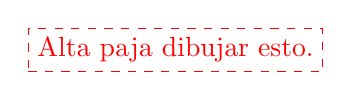
\begin{tikzpicture}
            \draw[red,dashed] (0,0) node[draw]{Alta paja dibujar esto.};
          \end{tikzpicture}
        \end{center}

        \[F_2=\SI{230}{\kilogram}\cdot\SI{9,80}{\meter\per\second\squared}=\SI{2,25e3}{\newton}\]

        \[P=\frac{F}{A}\land P_1=P_2\implies\frac{F_1}{A_1}=\frac{F_2}{A_2}\]
        \[\frac{F_1}{\pi\cdot(\SI{0,125}{in})^2}=\frac{\SI{2,25e3}{\newton}}{\pi\cdot(\SI{0,75}{in})^2}\]
        \[F_1=\frac{\SI{2,25e3}{\newton}}{\pi\cdot(\SI{0,75}{in})^2}\cdot\pi\cdot(\SI{0,125}{in})^2\]
        \[F_1=\SI{2,25e3}{\newton}\cdot\frac{\pi\cdot(\SI{0,125}{in})^2}{\pi\cdot(\SI{0,75}{in})^2}\]
        \[F_1=\SI{2,25e3}{\newton}\cdot\num{0,028}\]
        \[F_1=\SI{63,0}{\newton}\]
\end{enumerate}
\end{document}
